\documentclass{sig-alternate-05-2015}

\usepackage{hyperref}
\usepackage{xcolor}

\hypersetup{
    colorlinks,
    linkcolor={red!50!black},
    citecolor={blue!50!black},
    urlcolor={blue!80!black}
}

\begin{document}
\title{Predicting Censorship on Weibo}

\numberofauthors{2}
\author{
  \alignauthor
  Brian Tsay \\
  \email{brtsay@ucsd.edu}
  \alignauthor
  John Kuk \\
  \email{jskuk@ucsd.edu}
}

\date{1 December 2015}

\maketitle

% don't forget abstract
\begin{abstract}
  Put abstract here.
\end{abstract}


 \begin{CCSXML}
<ccs2012>
<concept>
<concept_id>10010405.10010455</concept_id>
<concept_desc>Applied computing~Law, social and behavioral sciences</concept_desc>
<concept_significance>300</concept_significance>
</concept>
</ccs2012>
\end{CCSXML}

\ccsdesc[300]{Applied computing~Law, social and behavioral sciences}
\printccsdesc

\section{Dataset} \label{sec:data}
% need time series plot
The data used for this assignment is taken from the \href{http://weiboscope.jmsc.hku.hk/datazip/}{Weiboscope} data collection and visualization project developed by the research team at the Journalism and Media Studies Centre, The University of Hong Kong \cite{Fu2013a}. The dataset consists of weibos (roughly the Chinese equivalent of tweets) collected in the year 2012. The authors created the dataset by first compiling a list of Weibo users with 1,000 or more followers and then getting their timelines, friends, and followers. Within the entire dataset, there are 226,841,122 tweets from 14,387,628 unique users. Of these tweets, 86,083 (about 0.03\%) are censored.

\begin{figure}
  \centering
  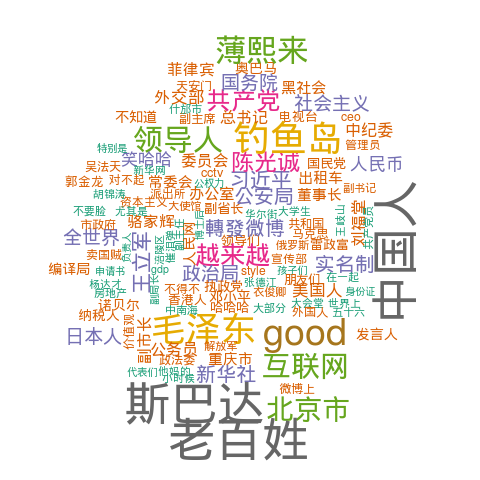
\includegraphics[scale = 0.52]{wordcloud_cens.png}
  \caption{Censored Tweets Word Cloud}
  \label{fig:wordcloud}
\end{figure}

Figure~\ref{fig:wordcloud} 

For the assignment, we kept all the censored tweets but kept only a small subsample (0.1\%) of the noncensored tweets. Noncensored tweets were randomly sampled from the entire dataset such that the number of noncensored tweets would be roughly twice that as the number of censored tweets within our data.\footnote{There was no particular reason that this ratio was chosen.} Whereas 0.03\% of tweets are censored in the entire dataset, 34\% of tweets are censored in our small subsample. The training set was constructed such that half of the tweets would be censored while the other half would be noncensored. The validation and test sets were deliberately constructed to look like one another. 

Table~\ref{tab:descript} shows some descriptive statistics for our dataset. It appears that more than half of the tweets in our subsample are retweets.\footnote{Note that this is a function of how the original dataset was constructed. This is not an artifact of our random sampling strategy.} We also see that, on average, each user is producing 2.5 tweets in our dataset. This implies that many tweets are correlated with one another. A retweet is very likely related to whatever the original tweet was, and individual users will probably tweet similar things over time. These aspects of the data will be incorporated into our features as described in Section~\ref{sec:pred}.

\begin{table*}
  \centering
  \begin{tabular}{|l|c|c|c|c|}
    \hline
    Statistic & Training Set & Validation Set & Test Set & Total \\
    \hline
    Retweets & 47930 & 41285 & 41414 & 130629 \\
    Unique Users & 39719 & 50446 & 50620 & 107907 \\
    \hline
    Censored Tweets & 43042 (50\%) & 21521 (25\%) & 21521 (25\%) & 86084 (34\%)  \\
    Non-censored Tweets & 43042 (50\%) & 63291 (75\%) & 63292 (75\% )& 169625 (66\%) \\
    Total Tweets & 86084 & 84812 & 84813 & 255709 \\
    \hline
  \end{tabular}
  \caption{Dataset Statistics}
  \label{tab:descript}
\end{table*}

\section{Predictive Task} \label{sec:pred}
We would like to predict which tweets are censored in this dataset i.e. a binary-class prediction. To evaluate our model, we will simply use classification accuracy -- the proportion of tweets that are labelled correctly. If we were Chinese government censors, then perhaps we would evaluate recall or $F_\beta$ instead.\footnote{Recall that $F_\beta = (1+\beta^2) \cdot \frac{\text{precision} \cdot \text{recall}}{\beta^2 \text{precision} + \text{recall}}$} The idea is that a government censor would prefer flagging a ``harmless'' tweet for censorship over accidentally letting a ``harmful'' tweet through. We are [fortunately] not Chinese government censors, so we will stick with evaluating our model using classification accuracy. Our data are split into training, validation, and test sets using the procedure described in Section~\ref{sec:pred}



\section{Model}

\section{Literature}

\section{Results}

\bibliographystyle{abbrv}
\bibliography{writeup}
\end{document}
